\documentclass{article}
\usepackage{graphicx}
\usepackage{wrapfig}
\usepackage{subcaption}
\usepackage[margin=1in]{geometry}
\usepackage{amsmath} % or simply amstext
\usepackage{siunitx}
\usepackage{booktabs}
\usepackage[export]{adjustbox}
\newcommand{\angstrom}{\textup{\AA}}
\newcommand{\colormap}{jet}  % colorbar to use
\usepackage{cleveref}
\usepackage{booktabs}
\usepackage{gensymb}
\usepackage{float}
\usepackage{xr}

\externaldocument[M-]{Draft}

\renewcommand{\thefigure}{S\arabic{figure}}
\renewcommand{\thesection}{S\arabic{section}}
\renewcommand{\thepage}{S\arabic{page}}
\renewcommand{\thetable}{S\arabic{table}}

\title{Supporting Information: Time Series Modeling of Solute Transport in an H\textsubscript{II} 
Phase Lyotropic Liquid Crystal Membrane}
\author{Benjamin J. Coscia \and Michael R. Shirts} 

\begin{document}

  \maketitle
  \graphicspath{{./supporting_figures/}}
  \bibliographystyle{ieeetr}
  
  \section{Setup and analysis scripts}\label{section:python_scripts}

  All python and bash scripts used to set up systems and conduct post-simulation trajectory
  analysis are available online at \texttt{https://github.com/shirtsgroup/LLC\_Membranes}.
  Documentation for the \texttt{LLC\_Membranes} repository is available at
  \texttt{https://llc-membranes.readthedocs.io/en/latest/}. Table~\ref{table:python_scripts}
  provides more detail about specific scripts used for each type of analysis performed in
  the main text.

  \begin{table}[htb!]
  \centering
  \newcolumntype{A}{ >{\centering\arraybackslash} m{2.5in} }
  \newcolumntype{B}{ >{\centering\arraybackslash} m{0.75in} }
  \newcolumntype{C}{m{2.75in}}
  \begin{tabular}{|A|B|C|}
  \hline
  \textbf{Script Name} & \textbf{Section} & ~~~~~~~~~~~~~~~~~~~~~\textbf{Description} \\
  \hline

  % mimic this
  \texttt{/setup/param.sh} & 2.1 & Parameterize liquid
  crystal monomers and solutes with GAFF \\ \hline

  \end{tabular}

  \caption{The first column provides the names of the python scripts available in
  the \texttt{LLC\_Membranes} GitHub repository that were used for system setup and
  post-simulation trajectory analysis. Paths preceding script names are relative to the
  \texttt{LLC\_Membranes/LLC\_Membranes} directory. The second columns lists the section in the main
  text where the output or usage of the script is first described. The third column
  gives a brief description of the purpose of each script.
  }~\label{table:python_scripts}

  \end{table}
  
  \section{Solute Equilibration}\label{section:equilibration}
  
  We collected all data used for model generation after the solutes were 
  equilibrated. We assumed a solute to be equilibrated when the partition of
  solutes in and out of the pore region stopped changing. The pore region is
  defined as within 0.75 nm of the pore center. We've plotted the partition
  versus time in Figure~\ref{fig:equilibration} and indicated the chosen
  equilibration time points.
  
  \begin{figure}
  \centering
  \begin{subfigure}{0.45\textwidth}
  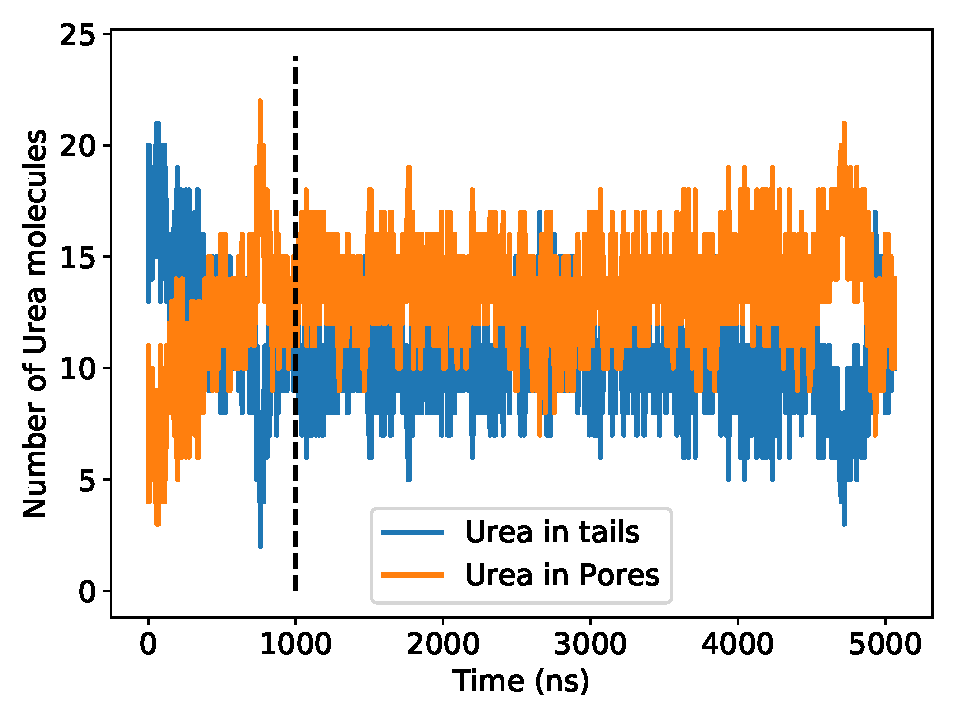
\includegraphics[width=\textwidth]{URE_equilibration.pdf}
  \caption{}\label{fig:URE_equilibration}
  \end{subfigure}
  \begin{subfigure}{0.45\textwidth}
  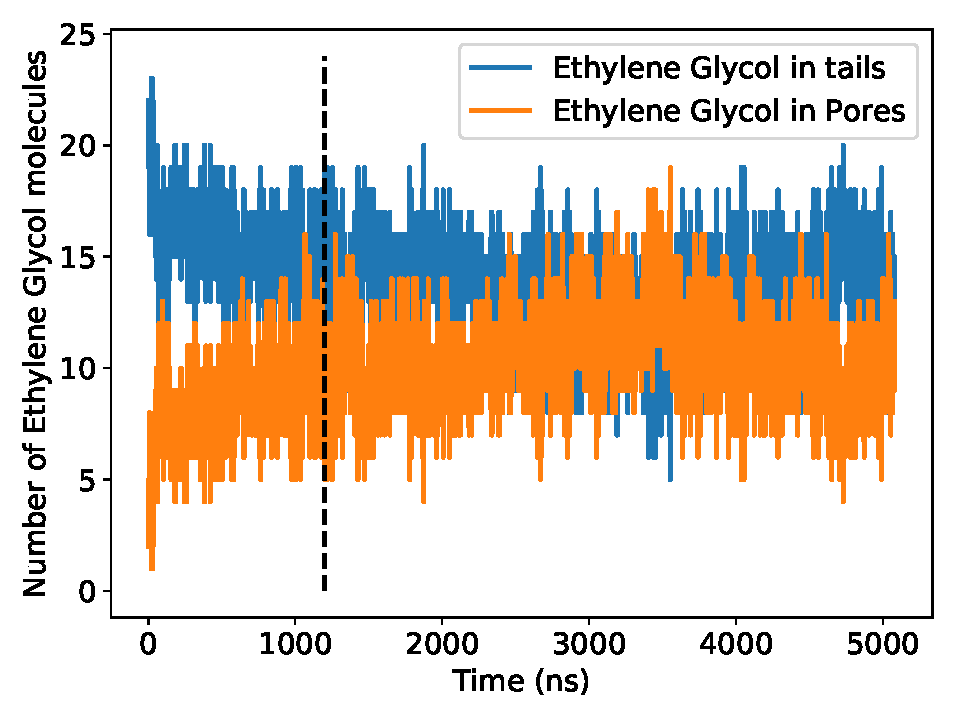
\includegraphics[width=\textwidth]{GCL_equilibration.pdf}
  \caption{}\label{fig:GCL_equilibration}
  \end{subfigure}
  \begin{subfigure}{0.45\textwidth}
  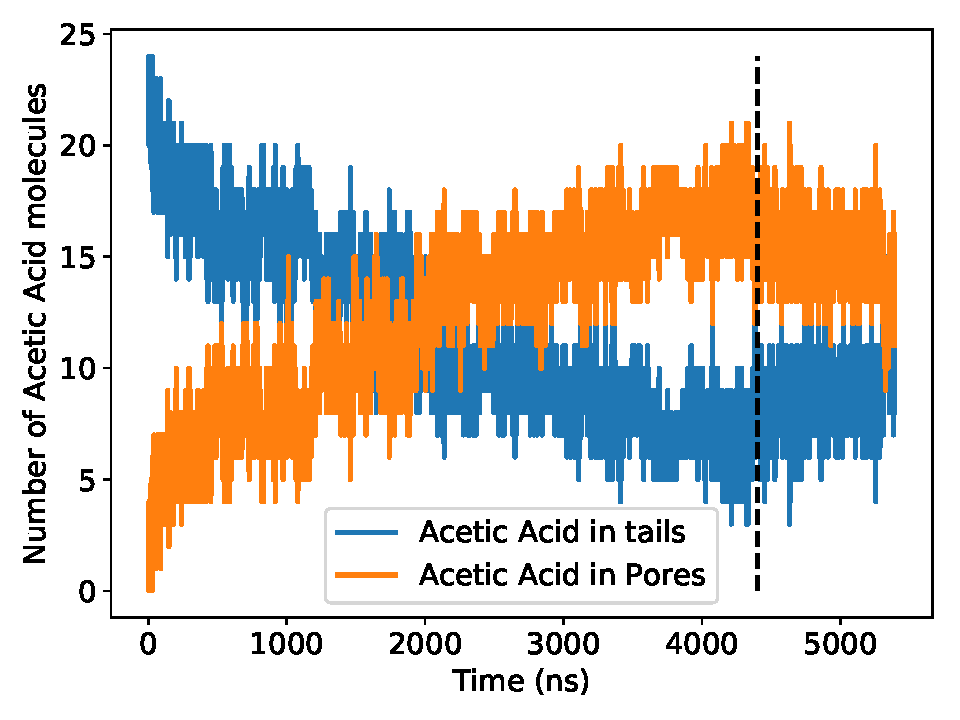
\includegraphics[width=\textwidth]{ACH_equilibration.pdf}
  \caption{}\label{fig:ACH_equilibration}
  \end{subfigure}
  \begin{subfigure}{0.45\textwidth}
  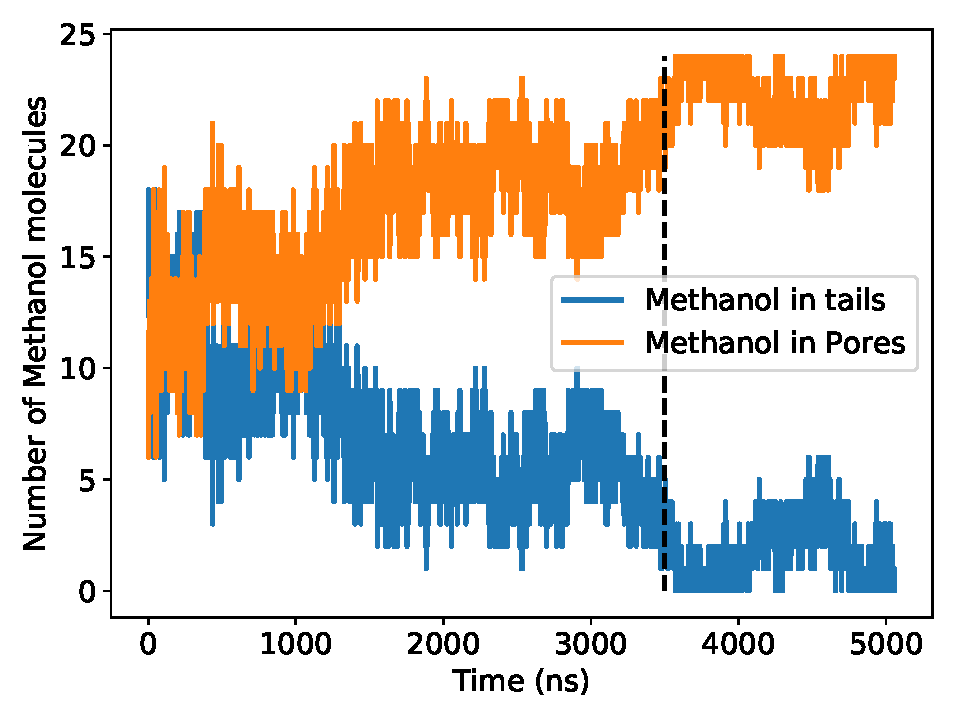
\includegraphics[width=\textwidth]{MET_equilibration.pdf}
  \caption{}\label{fig:MET_equilibration}
  \end{subfigure}
  \caption{We considered a system to be equilibrated when the partition of solutes
  between the tails and pore plateaued. Our chosen equilibration point for each
  solute is indicated by the vertical black dashed line. (a) Urea equilibrates
  the fastest, after 1000 ns. (b) Ethylene glycol equilibrates after 1200 ns 
  (c) Acetic Acid does not equilibrate until 4400 ns. (d) We considered methanol
  to be equilibrated after 3500 ns. Methanol nearly completely partitions into
  the tails.}\label{fig:equilibration}
  \end{figure}

%  \section{Choosing a transport model}\label{section:transport_model_selection}
%
%  We used the toolbox created by Meroz and Sokolov in order to justify our
%  choice of transport model.\cite{meroz_toolbox_2015} The solutes in our systems
%  exhibit anomalous transport properties characteristic of a Continuous Time
%  Random Walk (CTRW). 
%
%  \subsection*{Mean Squared Displacement}
%
%  The general form of a mean squared displacement (MSD) curve is:
%  \begin{equation}
%	\langle x^2(t) \rangle \sim t ^ \alpha
%	\label{eqn:msd}
%  \end{equation}
%  For brownian motion, $\alpha = 1$ and the MSD is linear. When $\alpha \neq
%  1$, the particle of interest exhibits anomalous diffusion. Values of $\alpha$
%  greater than 1 give rise to superdiffusion, while values of $\alpha$ less than
%  1 give rise to subdiffusion.
%
%  We can calculate the ensemble-averaged MSD curve by averaging the MSDs of
%  each particle trajectory, where each MSD is calculated using:
%  \begin{equation}
%	\delta^2(t) = \| \mathbf{r}(t) - \mathbf{r}(0) \|^2
%	\label{eqn:ensemble_msd}
%  \end{equation}
%  where $\|\cdot\|$ represents the Euclidean norm. 
%
%  The mean squared displacement of solutes in our model is a non-linear
%  function of time, with $\alpha < 1$ which is indicative of anomalous
%  subdiffusion. Figure \ref{fig:msd_power_law}a plots the ensemble-averaged MSD
%  curve for 24 ethanol molecules diffusing in a 10 wt\% water H\textsubscript{II}
%  LLC membrane system. We fit a power law of the form $Ae^{\alpha}$ to the MSD
%  curve. We performed 2000 bootstrap trials by randomly sampling 24 MSD curves
%  with replacement from the 24 total ethanol MSD curves. The bootstrapped average
%  value of $\alpha$ is 0.75 for this system. 
% 
%  \begin{figure}[!htb]
%  \centering
%% Generated with : msd.py -t PR_nojump.xtc -g PR.gro -r ETH -ensemble -power_law -a z -nboot 2000
%% in directory: /home/bcoscia/Documents/Gromacs/Transport/NaGA3C11/ETH/10wt
%  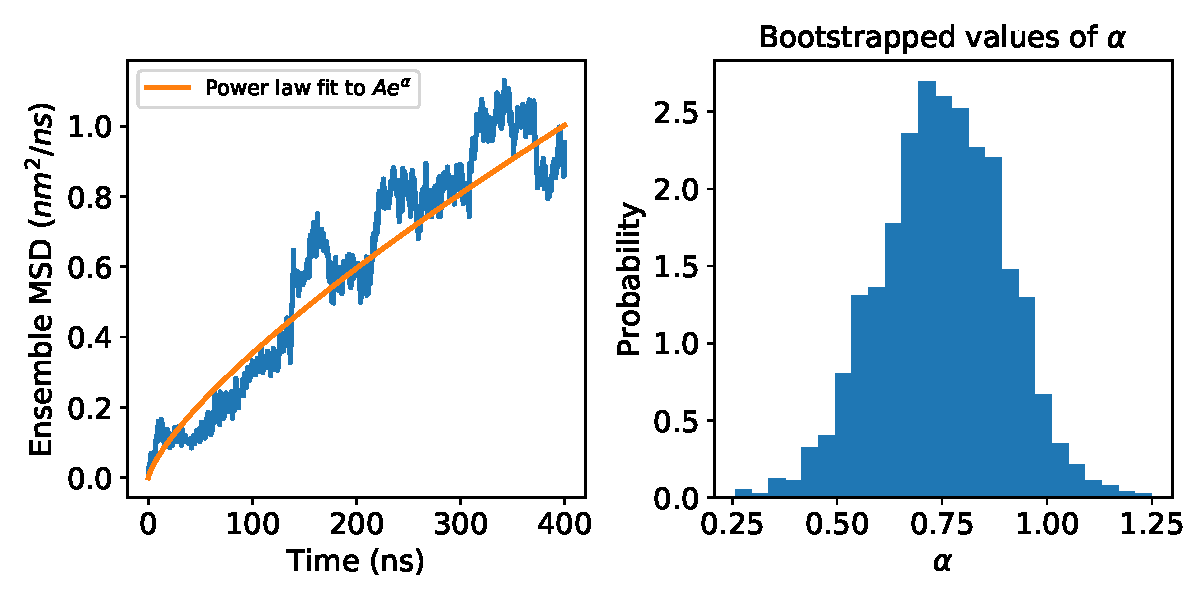
\includegraphics[width=0.8\linewidth]{msd_power_law.pdf}
%  \caption{(a) We fit a curve with the form of Equation~\ref{eqn:msd} to the
%	  ensemble-averaged MSD curve. (b) The average value of $\alpha$, obtained using
%	  fits to MSDs calculated from bootstrapped ensembles, is less than 1 suggesting
%	  that ethanol molecules in our model exhibit subdiffusive
%	  behavior.}\label{fig:msd_power_law}
%  \end{figure}
%
%  \subsection*{Ergodicity}
%
%  The ergodicity of a system can help us narrow down the possible anomalous
%  diffusion mechanisms. In an ergodic system, the time-averaged behavior of an
%  observable should yield the same result as the ensemble average of the same
%  observable. Examples of anomalous diffusion processes that are ergodic include
%  random walks on fractals (RWF) and fractional brownian motion (FBM).
%  Non-ergodic systems generally give rise to CTRWs with the possibility of
%  combination with a RWF and/or FBM.\cite{meroz_toolbox_2015} 
%
%  We tested the ergodicity of our system by comparing the ensemble-averaged
%  and time-averaged MSD curves. We calculated the MSD of each ethanol trajectory
%  using Equation~\ref{eqn:ensemble_msd} and a time-averaged algorithm: 
%  \begin{equation}
%	\delta^2(t) = \dfrac{1}{N-t} \sum_{i=0}^{N-t-1} \| \mathbf{r}(i + t) - \mathbf{r}(i) \|^2
%  \end{equation}
%  where N is the total number of simulation frames, and t represents the length
%  of subinterval or number of frames per subinterval. We averaged the MSD curves
%  from each trajectory in order to create final MSD plots.
%
%  The ethanol molecules exhibit non-ergodic behavior because their
%  time-averaged and ensemble-averaged MSDs do not agree with each other
%  (Figure~\ref{fig:ethanol_msd_comparison}). We validated our analysis using a 1
%  ns simulation of a box of tip3p water molecules. As expected, since the
%  particles exhibit Brownian motion, the time-averaged and ensemble-averaged MSDs
%  agree with each within error (Figure~\ref{fig:water_box_msd_comparison}).
%
%  \begin{figure}[!htb]
%  \centering
%  \begin{subfigure}{0.45\textwidth}
%% Generated with : msd.py -t PR_nojump.xtc -g PR.gro -r ETH -compare -nboot 2000 -a z
%% in directory: /home/bcoscia/Documents/Gromacs/Transport/NaGA3C11/ETH/10wt
%  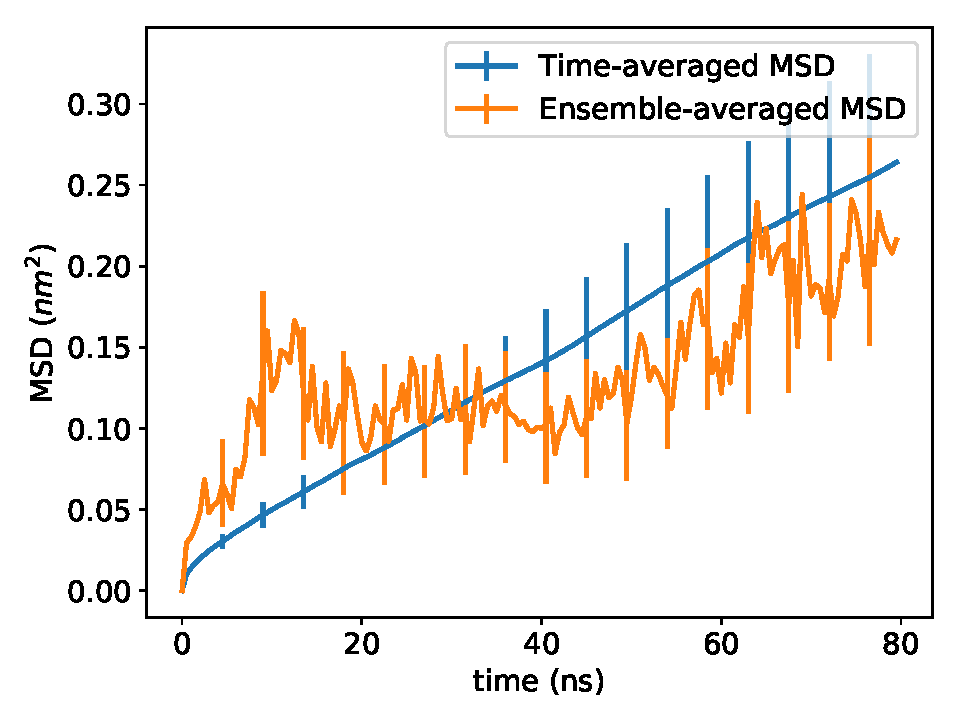
\includegraphics[width=\textwidth]{ethanol_msd_comparison.pdf}
%  \caption{}\label{fig:ethanol_msd_comparison}
%  \end{subfigure} 
%  \begin{subfigure}{0.45\textwidth}
%% Generated with msd.py -t traj_nojump.xtc -g npt.gro -r SOL -compare --fracshow 0.4 -nboot 2000 -a z
%% in directory: /home/bcoscia/Documents/Gromacs/Transport/Solvent/solvent_boxes/pure_water
%  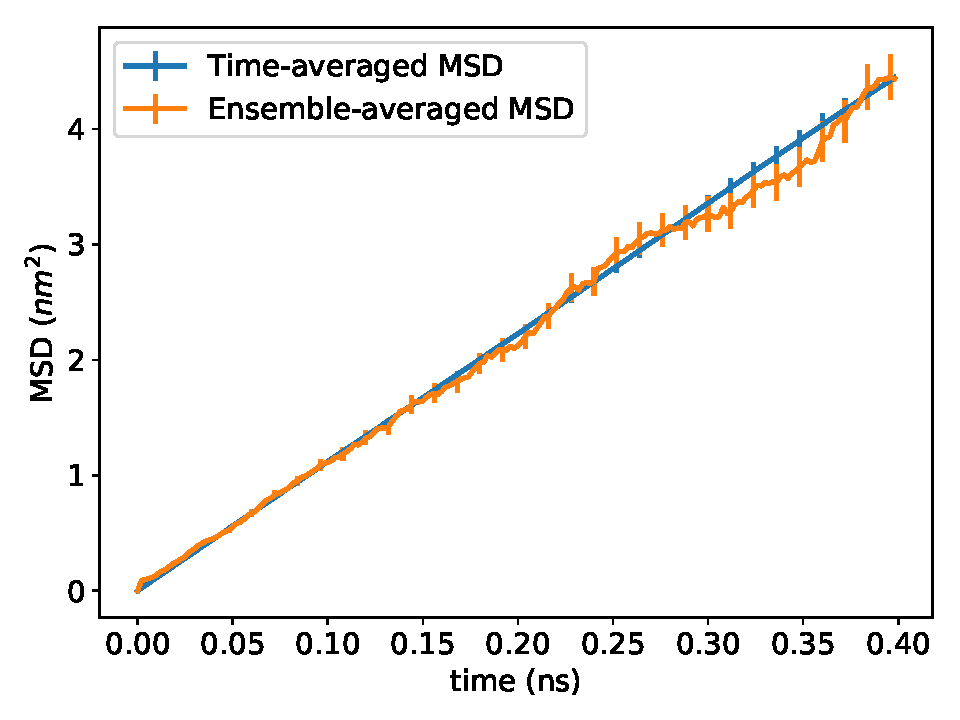
\includegraphics[width=\textwidth]{water_box_msd_comparison.pdf}
%  \caption{}\label{fig:water_box_msd_comparison}
%  \end{subfigure} 
%  \caption{(a) The time-averaged and the ensemble-averaged MSDs for ethanol in
%	  an H\textsubscript{II} nanopore are not in agreement, implying non-ergodicity.
%	  (b) A box of tip3p water molecules is expected to be ergodic and it is shown to
%	  be true here because both MSDs are in agreement. }\label{fig:msd_comparison}
%  \end{figure}

  
  \newpage
  \section{Estimating the Hurst Parameter}\label{section:H_estimate}
  
  We chose to estimate the Hurst parameter, $H$ by a least squares fit to the analytical
  autocorrelation function for fractional Brownian motion (the variance-normalized version 
  of Equation~\ref{M-eqn:fbm_autocorrelation} in the main text):
  
  \begin{equation}
    \gamma(k) = \dfrac{1}{2}\bigg[|k-1|^{2H} - 2|k|^{2H} + |k+1|^{2H}\bigg]
  \label{eqn:fbm_autocorrelation}
  \end{equation}  
  
  In Figure~\ref{fig:hurst_autocorrelation}, we plotted Equation~\ref{eqn:fbm_autocorrelation}
  for different values of $H$. When $H > 0.5$, Equation~\ref{eqn:fbm_autocorrelation} decays
  slowly to zero meaning one needs to study large time lags with high frequency in order to
  accurately estimate $H$ from the data. Fortunately, all of our solutes show anti-correlated
  motion, so most of the information in Equation \ref{eqn:fbm_autocorrelation} is contained
  within the first few lags. 

  % /supporting_figures/hurst_autocorrelation.py
  \begin{figure}
  \centering
  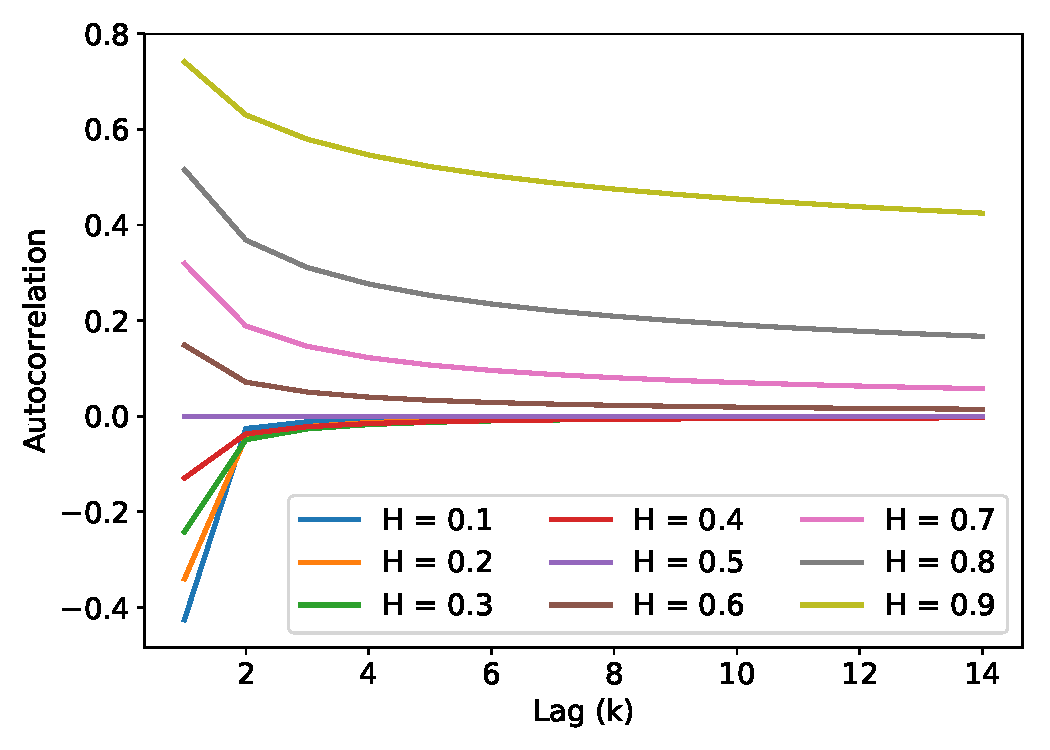
\includegraphics[width=0.5\textwidth]{hurst_autocorrelation.pdf}
  \caption{The analytical autocorrelation function of FBM decays to zero faster when 
  H $<$ 0.5 compared to when H $>$ 0.5.}\label{fig:hurst_autocorrelation}
  \end{figure}
  
  The autocovariance function of fractional L\'evy motion is different from fractional
  Brownian motion (see Equations~\ref{M-eqn:fbm_autocorrelation}
  and~\ref{M-eqn:flm_autocovariance} of the main text), but their autocorrelation 
  structures are the same. The autocovariance function of FLM is dependent on the 
  expected value of squared draws from the underlying L\'evy distribution, $E\big[L(1)^2\big]$. 
  This is effectively the distribution's variance, which is undefined for most 
  L\'evy stable distributions due to their heavy tails. As a consequence, one should 
  expect $E\big[L(1)^2\big]$ to grow as more samples are drawn from the distribution
  with the autocovariance function responding accordingly. 
  However, we are only interested in the autocorrelation function. In order to predict
  the Hurst parameter from the autocorrelation function, we must show that it has 
  a well-defined structure and is independent of the coefficient in 
  Equation~\ref{M-eqn:flm_autocovariance} of the main text. In Figure~\ref{fig:flm_autocorrelation}, 
  we plot the average autocorrelation function from an FLM process with an increasing 
  number of observations per generated sequence. For all simulations we set $H$=0.35 
  and $\alpha$=1.4. The variance-normalized autocovariance function, i.e. the autocorrelation
  function, does not change with increasing sequence length. Additionally, the
  autocorrelation function of FBM, with the same $H$, is the same.
  
  % supporting_figures/flm_autocov.py
  \begin{figure}
  \centering
  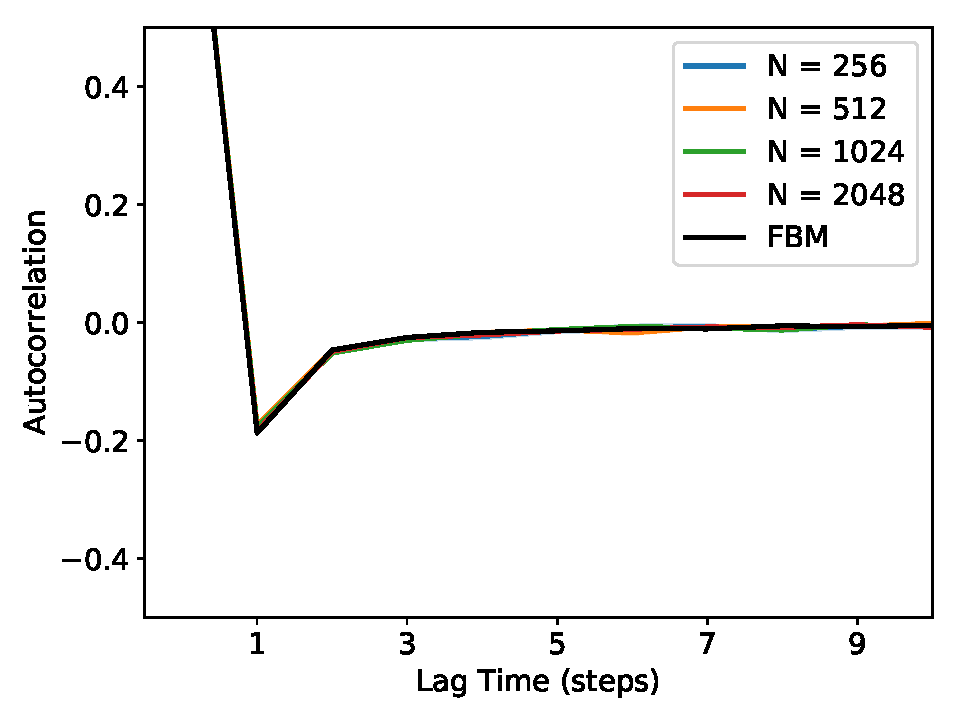
\includegraphics[width=0.5\textwidth]{flm_autocovariance.pdf}
  \caption{The autocorrelation function of an FLM process does not change with 
  increasing sequence length (N). It shares the same autocorrelation function as
  fractional Brownian motion (FBM). All sequenced used to make this plot were 
  generated using $H$=0.35 and, for FLM, $\alpha$=1.4.}\label{fig:flm_autocorrelation}
  \end{figure}
  
  \section{Simulating Fractional L\'evy Motion}\label{section:sFLM}

  \subsection{Truncated L\'evy stable hop distributions}\label{section:truncation}
  
  \textit{Determining where to truncate the hop distribution:} A pure
  L\'evy stable distribution has heavy tails which can lead to arbitrarily
  long hop lengths. Our distribution of hop lengths fits well to a L\'evy
  distribution near the mean, but under samples the tails. In 
  Figure~\ref{fig:truncation_correction} we compare the empirically 
  measured transition emission distribution of the MSDDM for Urea to its maximum likelihood fit to
  a L\'evy stable distribution. The ratio between the two distributions 
  at each bin is nearly 1 close to the center, indicating a near-perfect
  fit, larger than 1 slightly further from the center, suggesting that 
  we slightly over sample intermediate hop lengths, and below 1 far from 
  the center, indicating under sampling of extremely long hop lengths.
  Based on the plot, we chose a cut-off of 0.8 nm in order to compensate for
  over sampled intermediate hop lengths. We used the same procedure
  to determine truncation parameters for all solutes.
  
  \begin{figure}
  \centering
  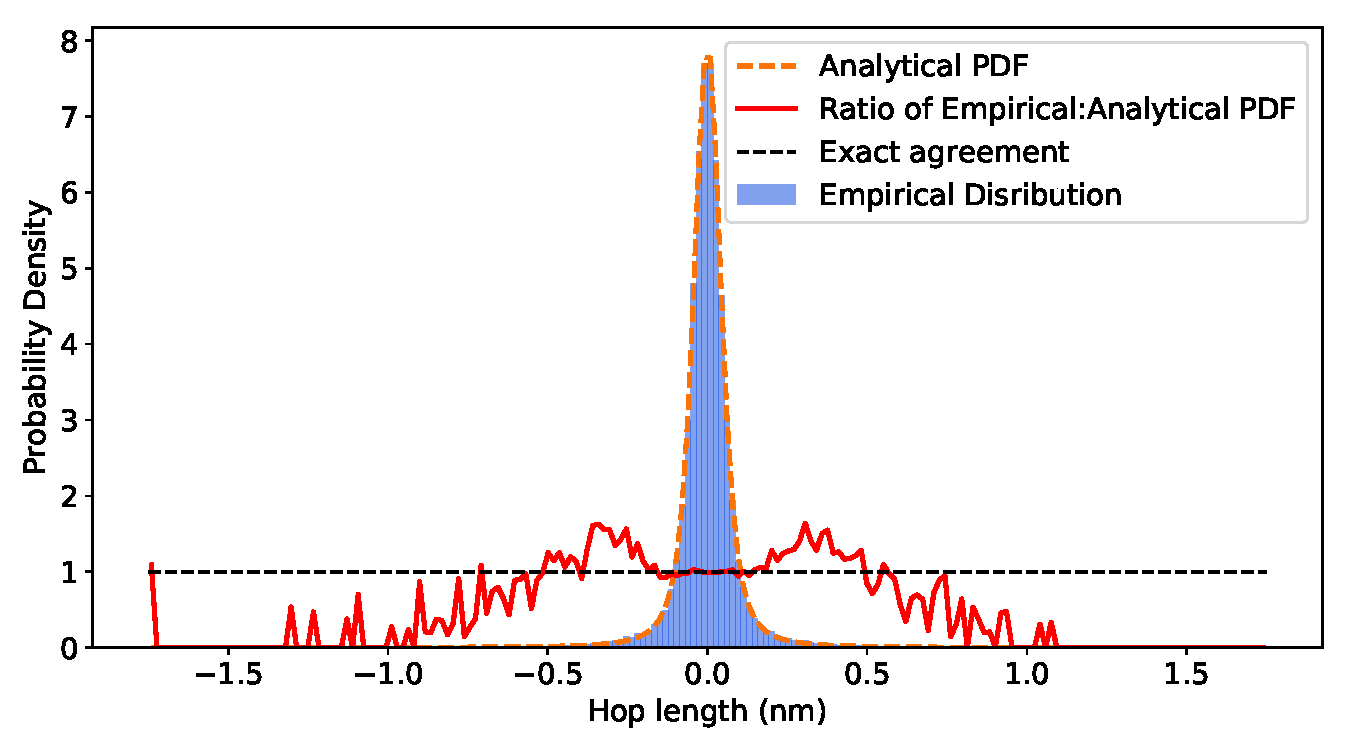
\includegraphics[width=0.75\textwidth]{truncation_cutoff.pdf}
  \caption{The ratio between the empirical and maximum likelihood theoretical
  distribution quantifies the quality of fit as function of hop length. The fit
  is near-perfect close to the mean. Intermediate hop lengths are over sampled, 
  and the tails are under sampled. We used this type of plot to determine the
  appropriate place to truncate the L\'evy stable distributions.}\label{fig:truncation_cutoff}
  \end{figure}
  
  \textit{Generating FLM realizations from a truncated L\'evy distribution:}
  To generate realizations from an uncorrelated truncated L\'evy process, one would
  randomly sample from the base distribution and replace values that are too large
  with new random samples from the base distribution, repeating the process until
  all samples are under the desired cut-off. 
  
  This procedure is complicated by the correlation structure of FLM. At a high level,
  Stoev and Taqqu use Riemann-sum approximations of the stochastic integrals defining
  FLM in order to generate realizations. They do this efficiently with the help of 
  Fast Fourier Transforms. In practice, this requires one to Fourier transform a zero-padded
  vector of random samples drawn from the appropriate L\'evy stable distribution, multiply
  the vector in Fourier space by a kernel function and invert back to real space. The end
  result is a correlated vector of fractional L\'evy noise.
  
  If one is to truncate an FLM process, one can apply the simple procedure above for 
  drawing uncorrelated values from the marginal L\'evy stable distribution, but after
  adding correlation, the maximum drawn value is typically lower than the limit set 
  by the user. Additionally, the shape of the distribution itself changes. Analogous
  to the database used to correct the Hurst parameter, we created a database to 
  correct the input truncation parameter (the maximum desired draw). The database
  returns the value of the truncation parameter that will properly truncate the
  output marginal distribution based on $H$, $\alpha$ and $\sigma$ (the width parameter).
  Figure~\ref{fig:truncation_correction} shows the result of applying our correction.
  Note that generating this database requires a significant amount of simulation and
  still likely doesn't perfectly correct the truncation parameter. The output leads
  to a somewhat fuzzy, rather than abrupt, cut-off of the output distribution. This 
  is likely beneficial since we observe a small proportion of hops longer the chosen
  truncation cut-off. When the cut-off value is close to the L\'evy stable $\sigma$ parameter,
  as it is in our anomalous diffusion models, we observed that the tails of the 
  truncated distribution tend to be undersampled. In order to maintain the distribution's 
  approximate shape up to the cut-off value we recommend ensuring that the cut-off
  value is at least 2 times $\sigma$. However, this may lead to a slight over-prediction
  of the MSD.
  
  \begin{figure}
  \centering
  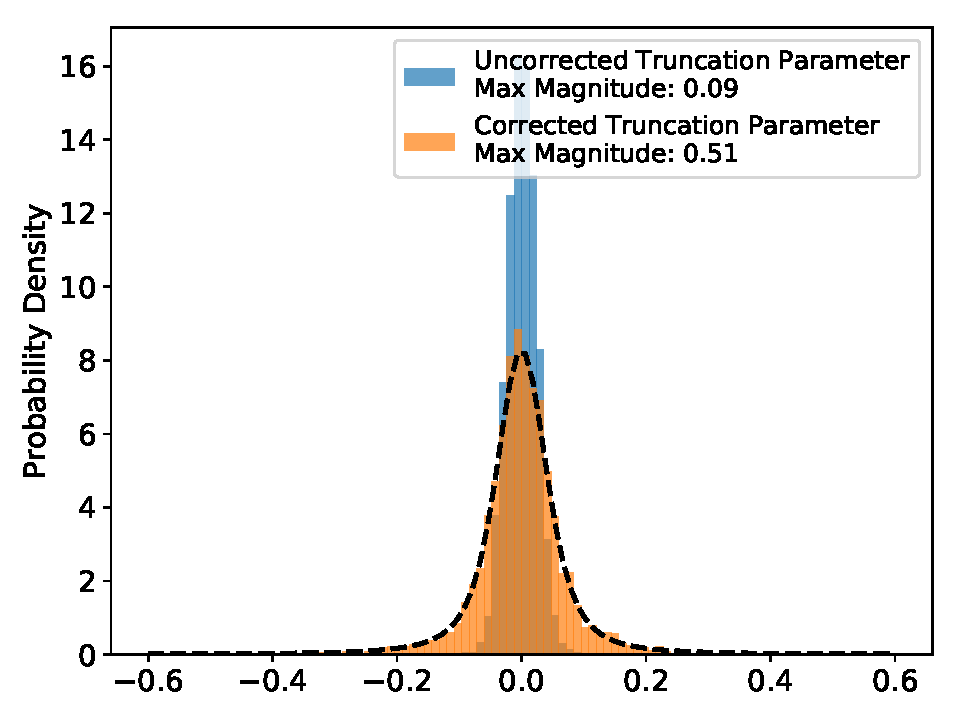
\includegraphics[width=0.5\textwidth]{truncation_correction.pdf}
  \caption{We can accurately truncate the marginal distribution of FLM innovations by
  applying a correction to the input truncation parameter. We generated FLM sequences
  and truncated the initial L\'evy stable distribution (before Fourier transforming) at 
  a value of 0.5. After correlation structure is added, the width of the distribution 
  of fractional L\'evy noise decreases significantly. We corrected the input truncation
  parameter with our database resulting in a distribution close to the theoretical
  distribution (black dashed line) with a maximum value close to 0.5.}\label{fig:truncation_correction}
  \end{figure}
  
  \subsection{Achieving the right correlation structure}\label{section:flm_correlation}
  
  We simulated FLM using the algorithm of Stoev and Taqqu~\cite{stoev_simulation_2004}.
  There are no known exact methods for simulating FLM. As a consequence, passing a
  value of $H$ and $\alpha$ to the algorithm does not necessarily result in the correct
  correlation structure, although the marginal L\'evy stable distribution is correct. 
  We applied a database-based empirical correction in order to use the
  algorithm to achieve the correct marginal distribution and correlation structure.
  
  Stoev and Taqqu note that the transition between negatively and positively correlated
  draws occurs when $H = 1/ \alpha$. When $\alpha=2$, the marginal distribution is 
  Gaussian and the transition occurs at $H=0.5$ as expected from FBM. We corrected 
  the input $H$ so that the value of $H$ measured based on the output sequence equaled
  the desired $H$. We first adjusted the value of $H$ by adding ($1 / \alpha - 0.5$),
  effectively recentering the correlation sign transition for any value of $1 \leq \alpha \leq 2$.
  This correction alone does a good job for input $H$ values near 0.5, but is
  insufficient if one desires a low value of $H$. The exact correction to $H$ is 
  not obvious so we created a database of output $H$ values tabulated as a function
  of input $H$ and $\alpha$ values. Figure~\ref{fig:hurst_correction} demonstrates the
  results of applying our correction. Without the correction, FLM realizations are
  more negatively correlated. This would result in under-predicted mean squared
  displacements when applying the model.
  
  % /supporting_figures/demonstrate_hurst_correction.py
  \begin{figure}
  \centering
  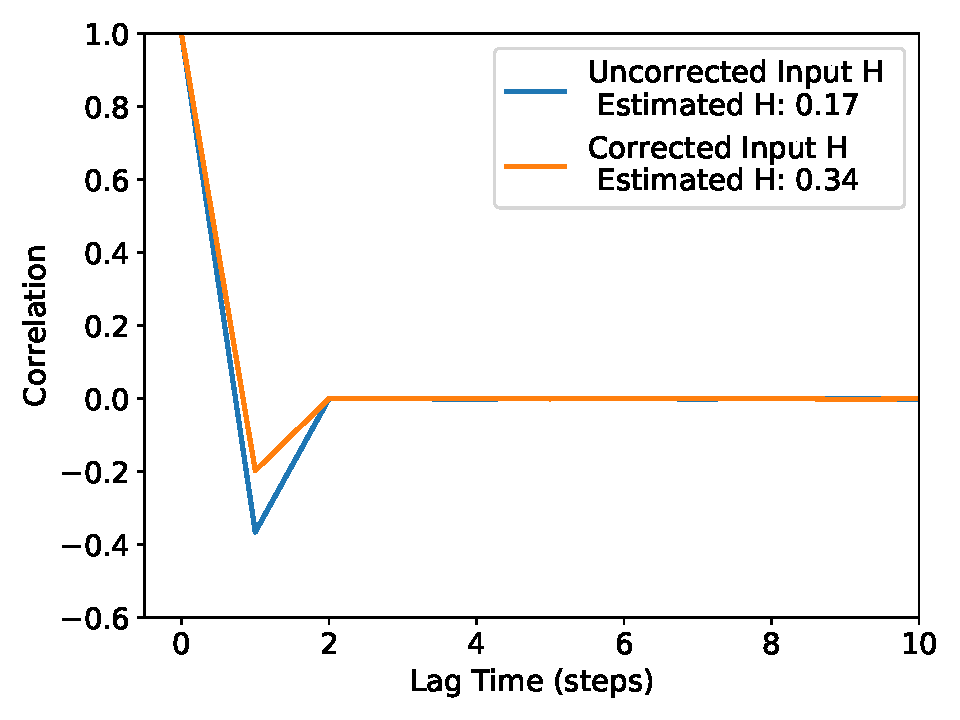
\includegraphics[width=0.5\textwidth]{hurst_correction.pdf}
  \caption{Correcting the Hurst parameter input to the algorithm of Stoev and Taqqu
  results in an FLM process with a more accurate correlation structure. We generated
  sequences with an input $H$ of 0.35. We estimated $H$ by fitting the autocorrelation
  function. Without the correction, $H$ is underestimated, meaning realizations are 
  more negatively correlated than they should be.}\label{fig:hurst_correction}
  \end{figure}
  
  \section{2-state MSDDM parameters}\label{section:simple_msddm_params}
  
  We used a simple 2-state model to illustrate how the self-transition probability 
  effects simulated MSDs generated from the MSDDM. We used the following parameters:
  
  \begin{table}[h]
  \centering
  \begin{tabular}{|c|c|c|c|}
  \hline
  State & H     & $\alpha_h$ & $\sigma$ \\\hline
  1     & 0.1  & 1.7       & 0.04    \\
  2     & 0.2  & 1.5       & 0.04    \\
  T     & 0.4  & 1.4       & 0.04    \\\hline
  \end{tabular}
  \caption{Values of $H$, $\alpha_h$ and $\sigma$ used to simulate realizations
  of the simple MSDDM whose MSDs are shown in Figure~\ref{M-fig:T_sensitivity} of
  the main text. The values are chosen to be similar to those in Table~\ref{M-table:msddm_params}
  of the main text.}\label{table:msddm_params}
  \end{table}

  \clearpage
  \bibliography{stochastic_transport}

\end{document}
